Consider 
\begin{align}
    \vec{A} = \myvec{a_1 \\ a_2 \\ a_3} 
\\
\vec{B} = \myvec{b_1 \\ b_2 \\ b_3} 
\end{align}
The cross product of the 2 matrices is,
\begin{align} \label{eq:solutions/1/2eq_1}
    \vec{A} \times \vec{B} = \myvec{0 & -a_3 & a_2 \\ a_3 & 0 & -a_1 \\ -a_2 & a_1 & 0} \myvec{b_1 \\ b_2 \\ b_3} 
\end{align} 
Substituting $a_3 = b_3 = 0$ in \eqref{eq:solutions/1/2eq_1} and simplifying,
\begin{align}
    \implies \vec{A} \times \vec{B} = \myvec{0 & a_1 \\ -a_2 & 0} \myvec{b_1 \\ b_2}
\end{align}
%\renewcommand{\thefigure}{1}
\begin{figure}[!ht] \label{fig:solutions/1/2triangle_abc}
\centering
\resizebox{\columnwidth}{!}{%\documentclass{standalone}
%
%\usepackage{tikz,pgf} %and any other packages or tikzlibraries your picture needs
%
%\begin{document}
%\resizebox{\columnwidth}{!}{
\begin{tikzpicture}
\draw (0,0) node[anchor=north]{$B (0,0)$}
  -- (2,4) node[anchor=west]{$A (a_1,a_2)$}
  -- (4,0) node[anchor=north]{$C (c_1,c_2)$}
  -- cycle;
\end{tikzpicture}
%}
%\end{document}
}
\caption{$\triangle ABC$ with B at origin}
\label{fig:solutions/1/2/one}
\end{figure} 
Considering three points $\vec{A},\vec{B},\vec{C}$ on a triangle and $\vec{B}$ at origin,
\begin{align}
    \vec{A} - \vec{B} = \vec{A} \label{eq:solutions/1/2eq_4}\\
    \vec{C} - \vec{B} = \vec{C} \label{eq:solutions/1/2eq_5}
\end{align}
Area of triangle is,
\begin{align} \label{eq:solutions/1/2eq_6a}
    Area(\triangle ABC) = \frac{1}{2}\norm{(\vec{A} - \vec{B}) \times (\vec{C} - \vec{B})}
\end{align}
Substituting \eqref{eq:solutions/1/2eq_4}, \eqref{eq:solutions/1/2eq_5} in \eqref{eq:solutions/1/2eq_6a},
\begin{align} \label{eq:solutions/1/2eq_6b}
    \implies Area(\triangle ABC) = \frac{1}{2}\norm{\vec{A} \times \vec{C}}
\end{align}
Constructing another triangle DBC with base as BC,
%\renewcommand{\thefigure}{2}
\begin{figure}[!ht] \label{fig:triangle_abc}
\centering
\resizebox{\columnwidth}{!}{%\documentclass{standalone}
%
%\usepackage{tikz,pgf} %and any other packages or tikzlibraries your picture needs
%
%\begin{document}
%\resizebox{6cm}{6cm}{
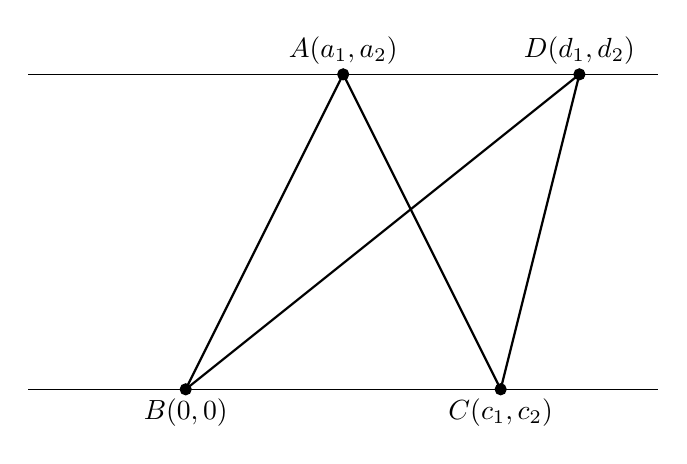
\begin{tikzpicture}
\draw (-2,0) -- (6,0); 
\draw (-2,4) -- (6,4);
\filldraw[black] (0,0) circle (2pt) node[anchor=north] {$B (0,0)$};
\filldraw[black] (2,4) circle (2pt) node[anchor=south] {$A (a_1,a_2)$};
\filldraw[black] (4,0) circle (2pt) node[anchor=north] {$C (c_1,c_2)$};
\filldraw[black] (5,4) circle (2pt) node[anchor=south] {$D (d_1,d_2)$};
\draw[black,thick] (0,0) -- (2,4);
\draw[black,thick] (4,0) -- (2,4);
\draw[black,thick] (0,0) -- (5,4);
\draw[black,thick] (4,0) -- (5,4);
\draw[black] (4,0) -- (0,0);

\end{tikzpicture}
%}
%\end{document}
}
\caption{$\triangle ABC$ and $\triangle DBC$ with BC as common base}
\label{fig:solutions/1/2/two}
\end{figure} \\
Since AD $\parallel$ BC,
\begin{align} \label{eq:solutions/1/2eq_7}
    \vec{A} - \vec{D} = k(\vec{B} - \vec{C})
\end{align}
Now calculating the area of $\triangle DBC$,
\begin{align} \label{eq:solutions/1/2eq_8}
    Area(\triangle DBC) = \frac{1}{2}\norm{(\vec{D} - \vec{B}) \times (\vec{C}- \vec{B})} 
\end{align}
Substituting \eqref{eq:solutions/1/2eq_7} in \eqref{eq:solutions/1/2eq_8},
\begin{align}
    \implies Area(\triangle DBC) = \frac{1}{2}\norm{ (\vec{A}-k( \vec{B}- \vec{C}))\times( \vec{C}- \vec{B})} \nonumber \\
    \implies Area(\triangle DBC) = \frac{1}{2}\norm{(\vec{A}+k \vec{C})\times  \vec{C} } \nonumber\\    (\because \vec{C}- \vec{B}= \vec{C})\nonumber \\
    \implies Area(\triangle DBC) =  \frac{1}{2}\norm{\vec{A}\times  \vec{C} } (\because \vec{A} \times \vec{A} = 0 ) \label{eq:solutions/1/2eq_9}
\end{align}
It can be observed that \eqref{eq:solutions/1/2eq_9} is same as \eqref{eq:solutions/1/2eq_6b}
Hence, triangles on the same base(or equal bases) and between the same parallels are equal in area.
